\documentclass{beamer}

\usepackage[main=english,finnish]{babel}
\usepackage{cmbright}
\usepackage{fontspec}
\usepackage{booktabs}
\usepackage{pifont}
\usepackage{dot2texi}
\usepackage{amsmath}

\newsavebox{\mysavebox}
\newlength{\myrest}

\DeclareMathOperator*{\argmax}{arg\,max}
\newcommand{\cmark}{\textcolor{red}{\ding{51}}}%
\newcommand{\xmark}{\textcolor{green}{\ding{55}}}%
\newcommand{\mtag}[1]{% \tag{<name>}
\mathchardef\mhyphen="2D % Define a "math hyphen"
\ensuremath{\langle{}#1\rangle{}}}
%\usepackage{polyglossia}
\setsansfont[Ligatures = TeX,
             BoldFont  = CMU Bright SemiBold,
             ItalicFont = CMU Bright Oblique,
            ]{CMU Bright Roman}
\setmainfont[Ligatures = TeX,
             BoldFont  = CMU Bright SemiBold,
             ItalicFont = CMU Bright Oblique,
            ]{CMU Bright Roman}
\setmonofont[Ligatures = TeX,
             BoldFont  = CMU Typewriter Text Bold,
             ItalicFont = CMU Typewriter Text Oblique,
            ]{CMU Typewriter Text}
\usetheme{Madrid}

\mode<presentation>
\setbeamercovered{transparent}
\setbeamertemplate{enumerate items}[default]
\setbeamertemplate{itemize items}[default]

\title[POS tagger internals]{Averaged perceptron tagger}
\institute[JYU]{University of Jyväskylä\\
\vspace{5mm}
\url{https://www.github.com/frankier/perceptron-tagger-slides/}}
\author[Frankie Robertson]{Frankie Robertson\texorpdfstring{\\
\href{mailto:frrobert@student.jyu.fi}{\texttt{frrobert@student.jyu.fi}}}{}}

\date{18th of July, 2016}

\titlegraphic{\vfill
\includegraphics[height=1.5cm]{null.pdf}
  \hfill
  
\includegraphics[height=1.5cm]{jyu.pdf}
}

\begin{document}

\section{Title}
\begin{frame}
  \titlepage{}
\end{frame}

\begin{frame}
\frametitle{Outline}
\begin{itemize}

  \item Averaged structured perceptron with beam search

  \item A DSL for features

  \item Results for Kazakh

\end{itemize}
\end{frame}

\begin{frame}
\frametitle{Averaged structured perceptron with beam search 1/2}
\begin{itemize}

  \item \textbf{Structured prediction} is breaking down prediction of a large
    structure into subproblems and using results from earlier stages in later
    stages (like dynamic programming). For POS tagging the simplest approach is
    to tag left to right.

  \item \textbf{The perceptron} stores a sparse linear vector of (feature,
    weight) pairs.  Observations are scored by taking the dot product of their
    feature vector with the perceptron. Training is done trying a prediction,
    and updating incorrect weights by reenforcing or penalising them depending
    on whether they correspond with the correct observation.

  \item With the \textbf{structured perceptron} the score from each update is
    accumulated to get the score of the (partial) output.

\end{itemize}
\end{frame}

\begin{frame}
\frametitle{Averaged structured perceptron with beam search 2/2}
\begin{itemize}

  \item The perceptron only converges for linearly separable inputs, otherwise
    its weights oscilate. To get the best weights the perceptron is trained for
    several iterations on reshuffled observations and the \textbf{averaged}
    weights across the whole training period are saved as the final weights.

  \item With \textbf{beam search}, the n-best candidates are considered and
    updated at each stage as opposed to a pure-greedy strategy which would only
    keep one intermediate result.

\end{itemize}
\end{frame}

{
\usebackgroundtemplate{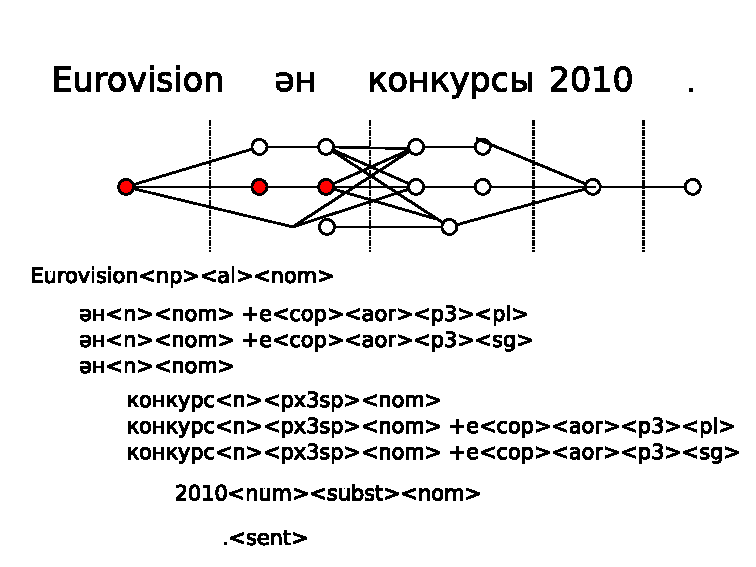
\includegraphics[width=\paperwidth]{update.pdf}}
\begin{frame}[plain]\end{frame}
}

\begin{frame}[fragile]
\frametitle{A DSL for features 1/3}

\begin{verbatim}
spectie: How's it going?

frankier: Been coding like a maniac

frankier: I've ended up creating a sort of lisp in XML
based on a stack VM

spectie: O\_\_\_O
\end{verbatim}

\end{frame}

\begin{frame}
\frametitle{A DSL for features 2/3}
\begin{center}
  
\includegraphics[height=7cm]{excuse-me-wtf-are-you-doing.jpg}
\end{center}
\end{frame}

\begin{frame}
\frametitle{A DSL 3/3}
\begin{itemize}

  \item Greenspun's tenth rule of programming: Any sufficiently complicated C
    or Fortran program contains an ad hoc, informally-specified, bug-ridden,
    slow implementation of half of Common Lisp.

  \item So why try to avoid it?

  \item Neither easy (for me) nor desirable to try and define every possible
    useful feature up front.

  \item Bytecode interpreter design is fasterand more modular than a tree
    walking interpreter and is usually the same or less code. Also it's easy to
    serialise.

  \item Hopefully empowers language authors more than it confuses them.

\end{itemize}
\end{frame}

\begin{frame}[fragile]
\frametitle{Example of DSL 1/2}
{\scriptsize
\begin{verbatim}
<def-global as="major_tag_0">
  <subscript idx="0">
    <ex-tags>
      <ex-wordoid><wrdaddr /></ex-wordoid>
    </ex-tags>
  </subscript>
</def-global>

<def-global as="is_dmorph">
  <streq val="+">
    <slice end="1">
      <ex-lemma>
        <ex-wordoid><wrdaddr /></ex-wordoid>
      </ex-lemma>
    </slice>
  </streq>
</def-global>
\end{verbatim}
}

\end{frame}

\begin{frame}[fragile]
\frametitle{Example of DSL 2/2}
{\scriptsize
\begin{verbatim}
<feat>
  <pred><var name="is_headword" /></pred>
  <out><var name="lemma_0" /></out>
  <out><var name="major_tag_0" /></out>
</feat>

<feat>
  <pred><var name="is_dmorph" /></pred>
  <out><var name="headword_major_tag_0" /></out>
  <out><var name="major_tag_0" /></out>
</feat>
\end{verbatim}
}

\end{frame}

\begin{frame}
\frametitle{Results}
Results!
\end{frame}

\begin{frame}
\frametitle{Future work}
\begin{itemize}

  \item Extend globals to macros/templates.

  \item Constructor for scanning/selecting a previous or subsequent wordoid or
    surface form or wordoid based on a predicate, eg to get the previous verb.

  \item Allow easy generation of multiple prefix/postfix features with special
    construct

\end{itemize}
\end{frame}

\begin{frame}
\frametitle{References}
\begin{itemize}

  \item Chinese segmentation. STAR Most helpful and similar to this implementation.

  \item Original Collins perceptron paper.

  \item \textit{\href{https://spacy.io/blog/part-of-speech-pos-tagger-in-python}{A Good Part-of-Speech Tagger in about 200 Lines of Python}},
    Matthew Honnibal, Blog Post.
    Plus: Easily understandable reference implementation. Minus: Formulation
    varies from rest of the literature.

\end{itemize}
\end{frame}

\end{document}
